\section{Redes neuronales y la toma de decisiones}
\subsection{El Modelo Biol\'{o}gico}
 
 		El sistema de procesamiento de informaci\'{o}n completo est\'{a} formado en
 		parte por el sistema nervioso central cuyo elemento principal es el cerebro,
 		\'{e}ste a su vez se encuentra compuesto por una unidad fundamental llamada \textit{neurona}.
 	\cite{Kriesel2005} La figura \ref{fig:neuronaBio} muestra las partes de la
 	neurona. En esta se puede observar la estructura t\'{i}pica de una neurona biol\'{o}gica, la
 	cual se encuentra formada por un cuerpo celular con su n\'{u}cleo o
 	\textit{soma}, del cual se desprende, en la parte superior, una serie de
 	ramificaciones denominadas \textit{dendritas}, mientras que en la parte
 	inferior se puede observar el \textit{ax\'{o}n}, \'{e}ste es una extensi\'{o}n del soma de forma tubular y
 	tiende a ramificarse en uno de sus extremos.
 	
 	\begin{figure}[htp]
 		\centering
 		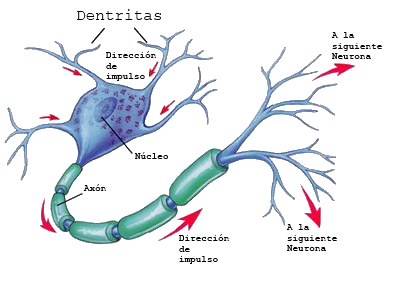
\includegraphics[width=0.5\textwidth]{images/TesisYGR-neuron.png}
 		\caption{Neurona Biol\'{o}gica}
 		\label{fig:neuronaBio}
 	\end{figure}
 	
 	 		Las neuronas son como cualquier otro tipo de c\'{e}lula, con la diferencia que
 	\'{e}stas pueden comunicarse entre s\'{i} \cite{Longo2011}. Por lo anterior, las dendritas
 	funcionan como un canal de entrada para recibir las se\~{n}ales que provienen del
 	exterior. Estas se\~{n}ales se transfieren a una neurona por medio de una conexi\'{o}n o contacto denominado sinapsis, mientras que el ax\'{o}n transfiere los pulsos hacia otras neuronas.

		Las se\~{n}ales entre las neuronas pueden ser de tipo el\'{e}ctrica o sinapsis
	el\'{e}ctrica que se da cuando la sinapsis recibe una se\~{n}al el\'{e}ctrica proveniente
	de una neurona transmisora o neurona pre sin\'{a}ptica y este es transmitido al
	n\'{u}cleo de la neurona receptora o pos sin\'{a}ptica. Por otro lado la
	sinapsis qu\'{i}mica se distingue por no presentarse un contacto el\'{e}ctrico
	entre ambas partes ya que este se interrumpe por causa de un abismo o grieta sin\'{a}ptico que separa un lado del otro. No obstante la informaci\'{o}n siempre fluye debido a que la se\~{n}al el\'{e}ctrica en el lado pre sin\'{a}ptico de la grieta se convierte en una se\~{n}al qu\'{i}mica que atraviesa la grieta y luego se vuelve a convertir en el la receptor \cite{Kriesel2005}.
 	
 		Una caracter\'{i}stica adicional de la sinapsis es la intensidad con la que se
 	transmiten las se\~{n}ales ya que estas tienden a variar, siendo unas transferidas
 	con fuerte estimulaci\'{o}n mientras que otras de forma d\'{e}bil. Este ajuste
 	var\'{i}a permitiendo que la estructura del cerebro no se mantenga fija
 	formando conexiones m\'{a}s fuertes o d\'{e}biles seg\'{u}n se requieran ajustes.

 		Usando un punto de vista funcional, una neurona de forma aislada, se
 	constituye en un procesador b\'{a}sico de informaci\'{o}n que cuenta con secci\'{o}n para
 	entradas (dendritas), un \'{a}rea de procesamiento (n\'{u}cleo o soma) y secci\'{o}n de
 	salida. Conforme se aumenta el panorama y se incluyen m\'{a}s neuronas y las interconexiones entre estas, se obtiene una red de neuronas que usan la sinapsis para poder transmitir se\~{n}ales unas a otras.
 		
 		
